% ------------------------------------------------------------------------------
% Copyright (c) 2010, 2020 Contributors to the Eclipse Foundation
%
% See the NOTICE file(s) distributed with this work for additional
% information regarding copyright ownership.
%
% This program and the accompanying materials are made available under the terms
% of the MIT License which is available at https://opensource.org/licenses/MIT
%
% SPDX-License-Identifier: MIT
% ------------------------------------------------------------------------------
{\ttfamily
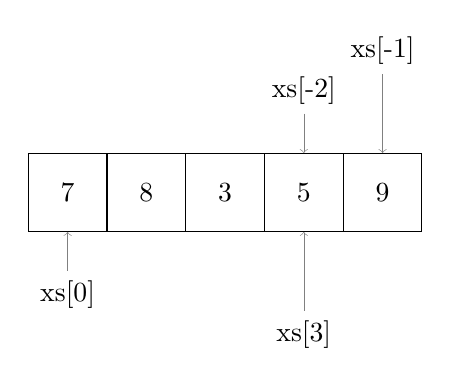
\begin{tikzpicture}[decoration=brace]
\draw (0,0) rectangle (1,1);
\draw (1,0) rectangle (2,1);
\draw (2,0) rectangle (3,1);
\draw (3,0) rectangle (4,1);
\draw (4,0) rectangle (5,1);
\draw (0.5,0.5) node {7};
\draw (1.5,0.5) node {8};
\draw (2.5,0.5) node {3};
\draw (3.5,0.5) node {5};
\draw (4.5,0.5) node {9};
\draw [<-,help lines] (0.5,0) -- (0.5,-0.5);
\draw (0.5,-0.8) node {xs[0]};
%\draw[decorate] (5,0) -- (1,0);
\draw [<-,help lines] (3.5,0) -- (3.5,-1);
\draw (3.5,-1.3) node {xs[3]};
\draw [->, help lines] (4.5,2) -- (4.5,1);
\draw (4.5, 2.3) node {xs[-1]};
%\draw [decorate] (0,1) -- (4,1);
\draw [->, help lines] (3.5,1.5) -- (3.5,1.0);
\draw (3.5, 1.8) node {xs[-2]};
\end{tikzpicture}
}
